
\textbf{


las 5 figuras, mas importantes + OJO unidades



extra: retrocohete
ley de pilotaje
cuerdo 3D con rotaciones al centro de masas

consultar trabajos reentrada atmosferica





1. introduccion
que es ballistic entry y como funciona (+ links de bibliogrtafia)
+ vehiculos de entrada sustentadors

2. Plateamineto de las ecuaciones dinámicas del mecanica de vuelo
(esquema página 16 ejes)

3. Esquema de cada imagen (x11)
- formulas + resolucion
- hipervinculo código matlab
- esquema ( con interpreter latex y diferentes tipos lineas)
- betas de capsulas reales (soyuz etc.)



$Libra_f$ = 
La libra (símbolos: lbf, o lbf), en física, es una unidad de fuerza. Una libra es aproximadamente igual a la fuerza gravitacional ejercida sobre una masa de una libra sobre una idealizada superficie de la Tierra. SOURCE = WIKIPEDIA

1 lbf ≡ 4,448222 newtons (kg·m/s²)

A Btu can be approximated as the heat produced by burning a single wooden kitchen match or as the amount of energy it takes to lift a one-pound (0.45 kg) weight 778 feet (237 m)

1 watt is approximately 3.412142 Btu/h 

A BTU was originally defined as the amount of heat required to raise the temperature of 1 avoirdupois pound of liquid water by 1 degree Fahrenheit at a constant pressure of one atmosphere.



%%% EXPRESSIÓ PRESSIO ESTANCAMENT
Reescrivint la calor específic com $C_p = \frac{\gamma R}{\gamma -1}$ i introduint la velocitat del so $a= \sqrt{\gamma R_g T}$ o el Mach es defineix com (\ref{eq:mach}):
\begin{equation*}
    \frac{T}{T_0} = 1 + \frac{\gamma - 1}{2} M^2
\end{equation*}
Aplicant la relació isentròpica,
\begin{equation*}
    \frac{p}{\rho^\gamma} = \mathrm{const} \hspace{7mm} i \hspace{7mm} \frac{p}{T^{\frac{\gamma}{\gamma -1 }}}
\end{equation*}
S'obté que la pressió d'estancament s'expressa de la següent forma:
\begin{equation}
    \frac{p_0}{p} = \left( 1 + \frac{\gamma - 1}{2} M^2\right)^\frac{\gamma}{\gamma - 1}
\end{equation}






%%
\url{https://www.quora.com/In-regards-to-atmospheric-reentry-what-exactly-is-a-ballistic-reentry-and-can-you-describe-in-detail-an-example-of-it}
fact sheet
\url{https://nssdc.gsfc.nasa.gov/planetary/factsheet/marsfact.html}
\url{https://nssdc.gsfc.nasa.gov/planetary/factsheet/earthfact.html}

%% 
EVERNOTE
\url{}

US STANDARD ATMOSPHERE NASA
\url{https://ntrs.nasa.gov/archive/nasa/casi.ntrs.nasa.gov/19770009539.pdf}


pagina web de codigo matlab
\url{https://es.mathworks.com/matlabcentral/fileexchange/28135-standard-atmosphere-functions}

Referencia de las ecuaciones
\url{http://www.pdas.com/atmos.html}
}








% fOTOS MERCURY
\newpage
\subsection{Gràfica: Velocitat respecte Altitud}

\begin{figure}[h]
    \centering
    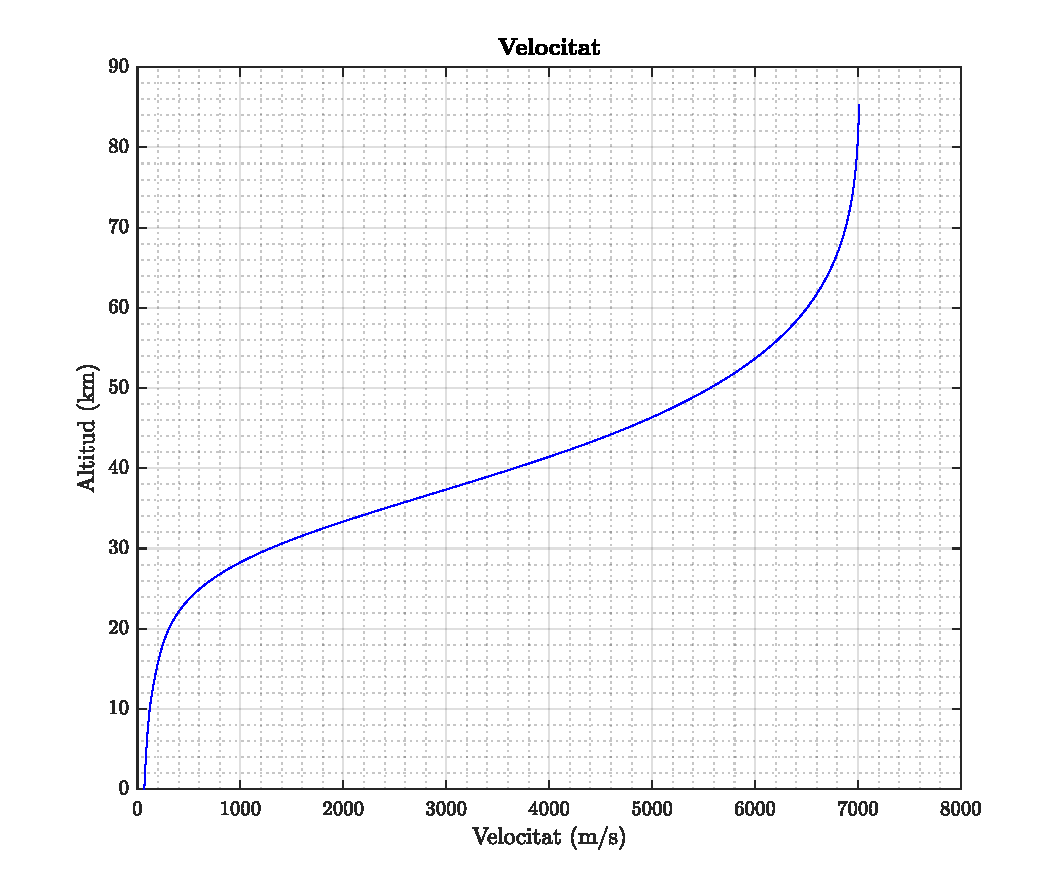
\includegraphics[width=0.75\textwidth]{imagenes/09_mercury_graficas/velocitat.pdf}
    \caption{Representació gràfica de la velocitat $V$ respecte l'alçada $h$ del ``Friendship 7''}
    \label{fig:velocitat_merc}
\end{figure}


\newpage
\subsection{Gràfica: Temps d'entrada respecte Altitud}

\begin{figure}[h]
    \centering
    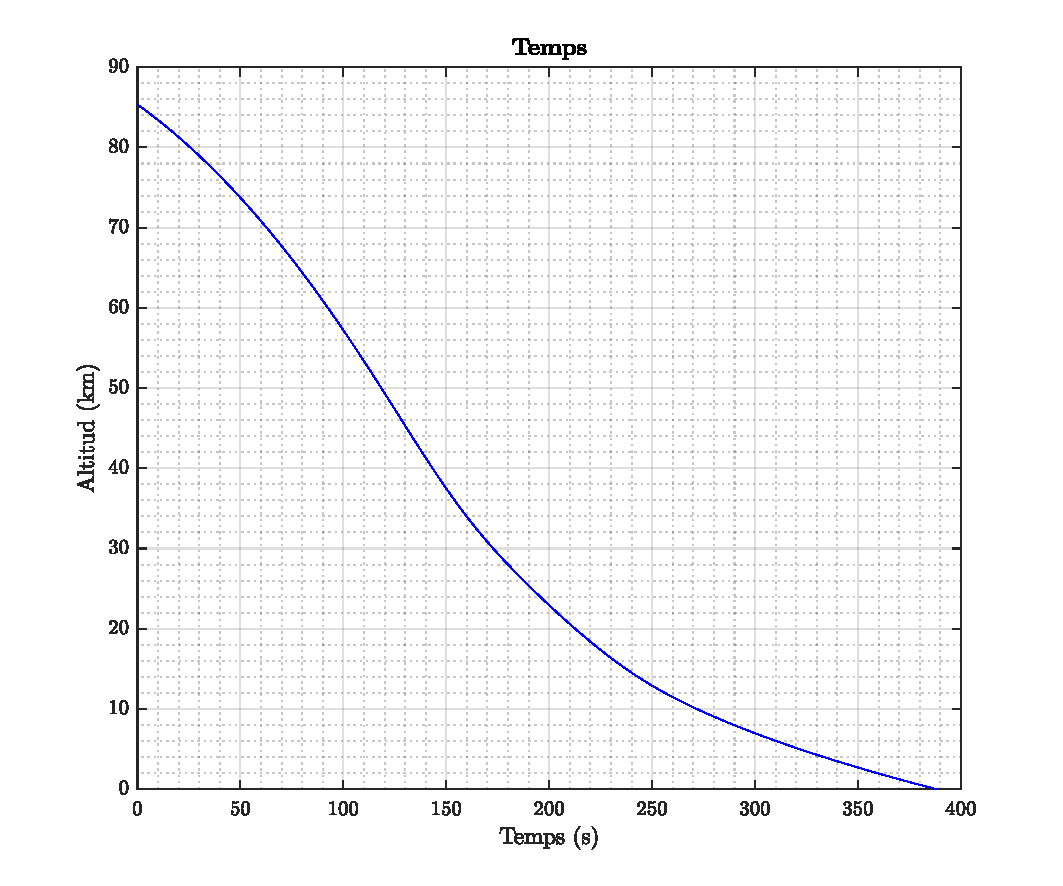
\includegraphics[width=0.75\textwidth]{imagenes/09_mercury_graficas/temps.pdf}
    \caption{Representació gràfica del temps de reentrada $V$ respecte l'alçada $h$ del ``Friendship 7''}
    \label{fig:temps_merc}
\end{figure}


\newpage
\subsection{Gràfica: Abast respecte Altitud}

\begin{figure}[h]
    \centering
    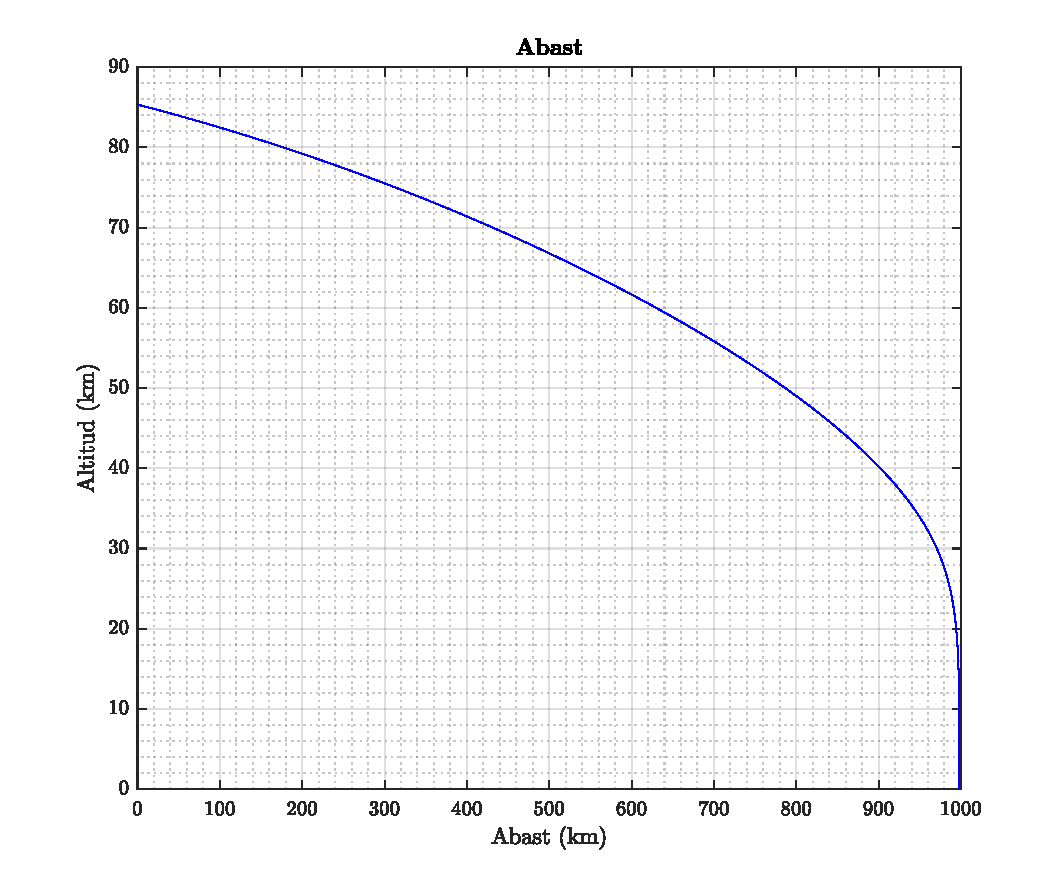
\includegraphics[width=0.75\textwidth]{imagenes/09_mercury_graficas/abast.pdf}
    \caption{Representació gràfica de l'abast $\Delta x$ respecte l'alçada $h$ del ``Friendship 7''}
    \label{fig:abas_merc}
\end{figure}


\newpage
\subsection{Gràfica: Desacceleració respecte Altitud}

\begin{figure}[h]
    \centering
    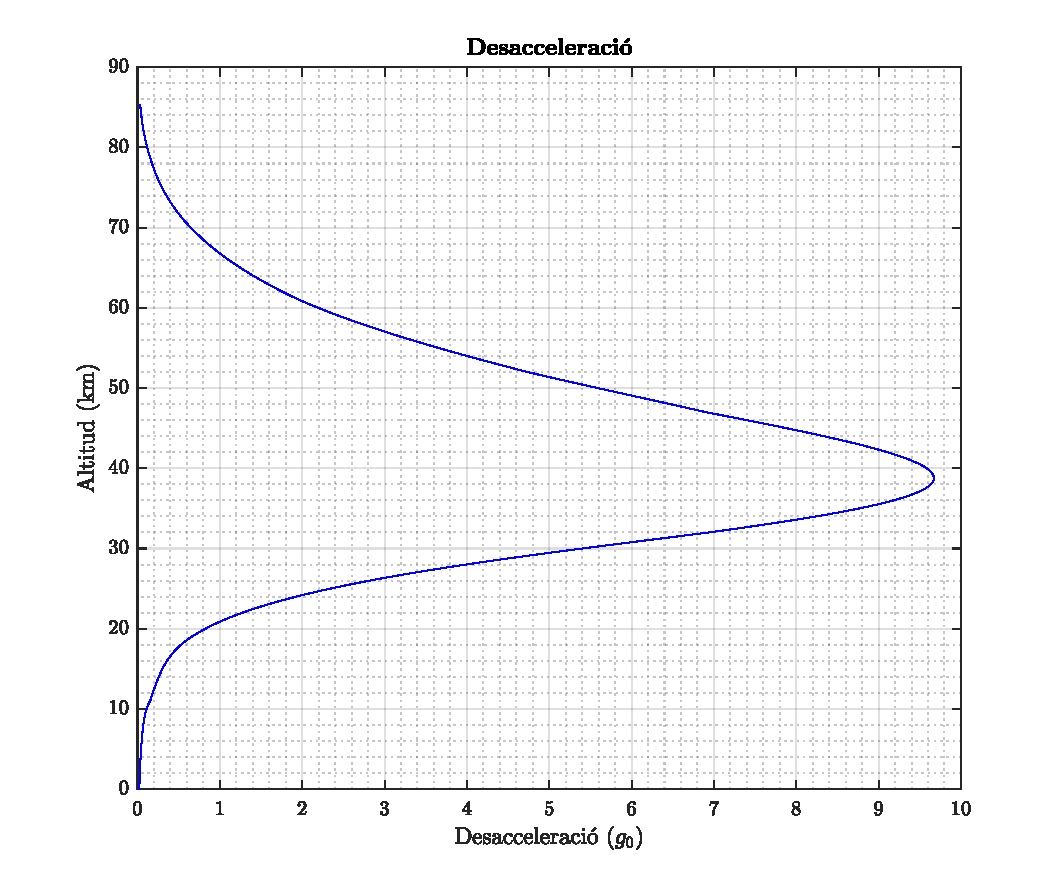
\includegraphics[width=0.75\textwidth]{imagenes/09_mercury_graficas/desacceleracio.pdf}
    \caption{Representació gràfica de la desacceleració $a$ respecte l'alçada $h$ del ``Friendship 7''}
    \label{fig:desacceleracio_merc}
\end{figure}


\newpage
\subsection{Gràfica: Número de Mach respecte Altitud}

\begin{figure}[h]
    \centering
    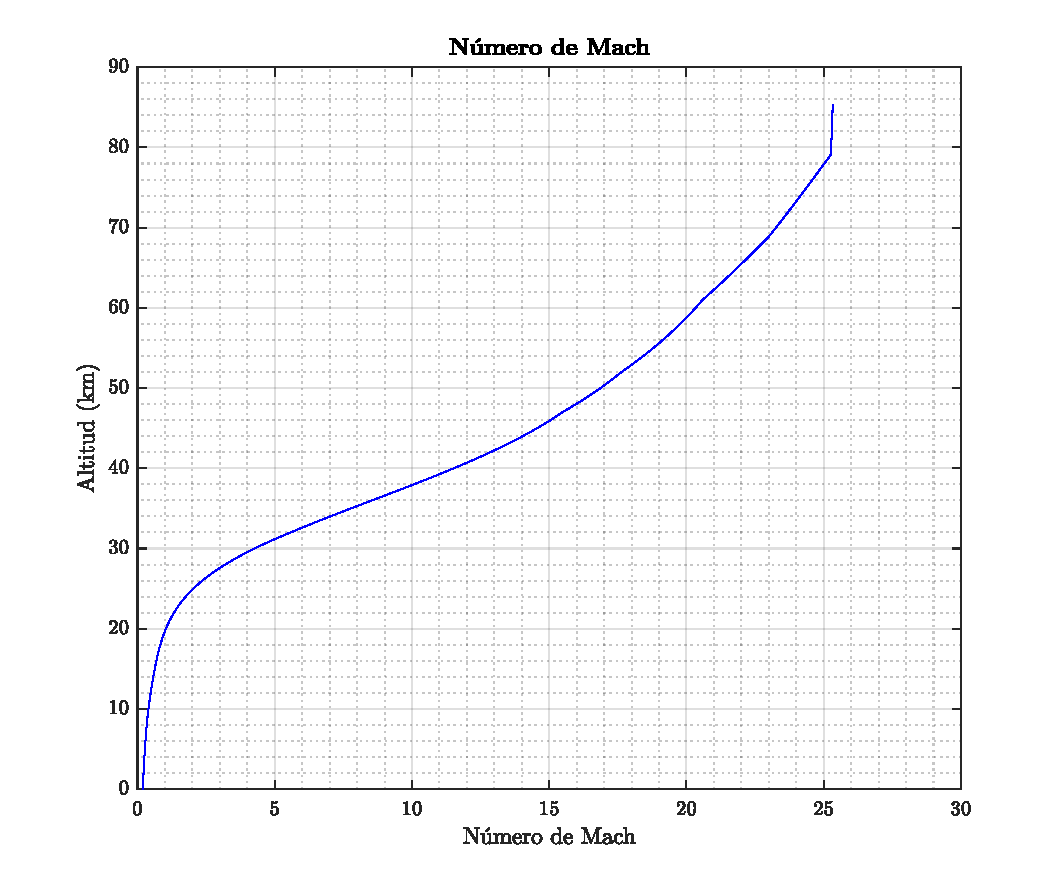
\includegraphics[width=0.75\textwidth]{imagenes/09_mercury_graficas/mach.pdf}
    \caption{Representació gràfica del número de Mach $M$ respecte l'alçada $h$ del ``Friendship 7''}
    \label{fig:mach_merc}
\end{figure}
